% --------------------------------------------------------------
% This is all preamble stuff that you don't have to worry about.
% Head down to where it says "Start here"
% --------------------------------------------------------------
 
\documentclass[12pt]{article}
 
\usepackage[margin=1in]{geometry} 
\usepackage{amsmath,amsthm,amssymb,scrextend}
\usepackage{fancyhdr}
\usepackage{enumitem}
\usepackage{amsmath}
\usepackage{amssymb}
\usepackage{textcomp}
\usepackage{fancybox}
\usepackage{tikz}
\usepackage{tasks}
\pagestyle{fancy}
\usepackage[makeroom]{cancel}
\usepackage{graphicx}
\usepackage{caption}
\usepackage{mwe}
\usepackage{tikz}
\usetikzlibrary{positioning}

\newcommand{\N}{\mathbb{N}}
\newcommand{\Z}{\mathbb{Z}}
\newcommand{\I}{\mathbb{I}}
\newcommand{\R}{\mathbb{R}}
\newcommand{\Q}{\mathbb{Q}}
\renewcommand{\qed}{\hfill$\blacksquare$}
\let\newproof\proof
\renewenvironment{proof}{\begin{addmargin}[1em]{0em}\begin{newproof}}{\end{newproof}\end{addmargin}\qed}
% \newcommand{\expl}[1]{\text{\hfill[#1]}$}
 
\newenvironment{theorem}[2][Theorem]{\begin{trivlist}
\item[\hskip \labelsep {\bfseries #1}\hskip \labelsep {\bfseries #2.}]}{\end{trivlist}}
\newenvironment{lemma}[2][Lemma]{\begin{trivlist}
\item[\hskip \labelsep {\bfseries #1}\hskip \labelsep {\bfseries #2.}]}{\end{trivlist}}
\newenvironment{problem}[2][Problem]{\begin{trivlist}
\item[\hskip \labelsep {\bfseries #1}\hskip \labelsep {\bfseries #2.}]}{\end{trivlist}}
\newenvironment{exercise}[2][Exercise]{\begin{trivlist}
\item[\hskip \labelsep {\bfseries #1}\hskip \labelsep {\bfseries #2.}]}{\end{trivlist}}
\newenvironment{reflection}[2][Reflection]{\begin{trivlist}
\item[\hskip \labelsep {\bfseries #1}\hskip \labelsep {\bfseries #2.}]}{\end{trivlist}}
\newenvironment{proposition}[2][Proposition]{\begin{trivlist}
\item[\hskip \labelsep {\bfseries #1}\hskip \labelsep {\bfseries #2.}]}{\end{trivlist}}
\newenvironment{corollary}[2][Corollary]{\begin{trivlist}
\item[\hskip \labelsep {\bfseries #1}\hskip \labelsep {\bfseries #2.}]}{\end{trivlist}}
 
\setlength{\parindent}{0pt}
\begin{document}
 \settasks{
	counter-format=(tsk[r]),
	label-width=4ex
}
% --------------------------------------------------------------
%                         Start here
% --------------------------------------------------------------

\lhead{Math 632}
\chead{Homework 6}
\rhead{Meenmo Kang}

\noindent
\textbf{1.} Let $\{N(t):t\ge 0\}$ be a rate $\lambda$ Poisson process, $\{T_k\}_{k\ge 1}$ the arrival times of the process, and $\tau_k = T_k - T_{k-1}$ for $k\ge 1$ the interarrival times. Calculate the probabilities below. When unspecified non-negative integers $j$ and/or $k$ appear in the question, your answer should cover all possible cases. When units are used, suppose the time unit is second.
\begin{enumerate}[label=(\alph*)]
    \item $P(N(2) = j,\; N(5)=k)$
    \begin{enumerate}[label=(\roman*)]
    \item $j=k$
    $$
    \frac{P(N(2) = j)\cap P(N(5)=k)}{P(N(5)=k)}
    =\frac{P(N(2) = j)}{P(N(5)=j)}
    = \frac{ \left(e^{-2\lambda}\cdot \frac{(2\lambda)^j}{j!}\right)}
    {e^{-5\lambda}\cdot \frac{(5\lambda)^j}{j!}}
    = e^{3\lambda}\cdot \left(\frac{2}{5}\right)^j
    $$
    \item $0<j<k$
    $$\frac{P(N(2) = j)\cap P(N(5)=k)}{P(N(5)=k)}
    =\frac{P(N(2) = j)\cap P(N(5)-N(2)=k-j)}{P(N(5)=k)}
    $$
    $$    =\frac{
    \left(e^{-2\lambda}\cdot \frac{(2\lambda)^j}{j!}\right)\cdot \left(e^{-3\lambda}\cdot \frac{(3\lambda)^{k-j}}{(k-j)!} \right)  }    
    {e^{-5\lambda}\cdot \frac{(5\lambda)^k}{k!}}
    =\frac{\cancel{e^{-5\lambda}}\cdot \left(
    \frac{2^j\cdot 3^{k-j}\cdot \cancel{\lambda^k}}
    {\cancel{k!}}
    \right)}
    {{\cancel{e^{-5\lambda}}\cdot \frac{(5\cancel{\lambda})^k}{\cancel{k!}}}} = \frac{2^j\cdot 3^{k-j}}{5^k}    $$
    
    $$P(N(2) = j,\; N(5)=k)=
    \begin{cases}
    e^{3\lambda}\cdot \left(\frac{2}{5}\right)^j &\text{if } j= k\\
    \frac{2^j\cdot 3^{k-j}}{5^k} & \text{if } 0<j<k\\
    0 & \text{if } j\le 0
    \end{cases}
    $$
    \end{enumerate}
    
    \item P(after the 3rd arrival there are no arrivals for 20 seconds,\\ 
    \qquad but after that the next two arrivals come within 10 seconds)
    $$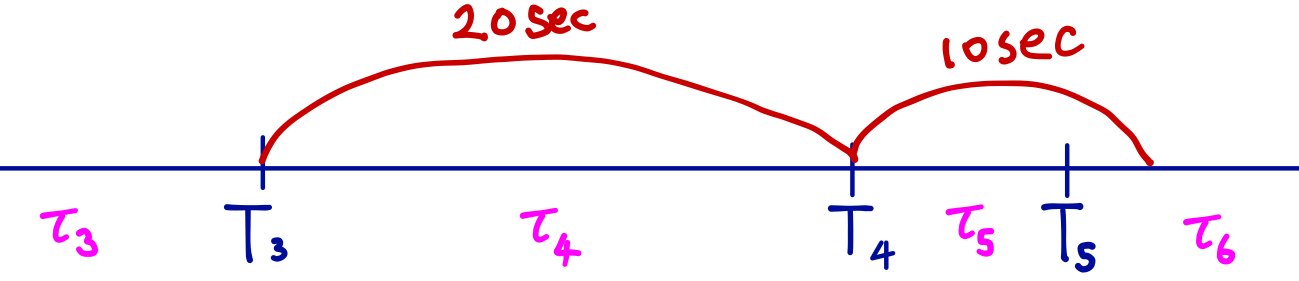
\includegraphics[height=1.4cm, width=12cm]{HW6/P1.jpeg}$$
    $$\text{No arrival for 20 seconds after $T_3$: }P(\tau_4 > 2) = P(N(2)=0) = e^{-2\lambda}\cdot \frac{(2\lambda)^0}{0!}=e^{-2\lambda}$$
    $$\text{Two arrivals within 10 seconds after $T_4$: }P(N(1)=2)= e^{-\lambda}\cdot \frac{\lambda^2}{2!}$$
    So the ultimate probability we are trying to get is
    $$e^{-2\lambda}\cdot e^{-\lambda}\cdot \frac{\lambda^2}{2!} = e^{-3\lambda}\cdot \frac{\lambda^2}{2!}$$
    \item $P(N(3)=k\;|\; T_2\le 3)$
    $$=    \frac{P(N(3)=k)\cap P(T_2\le 3)}{P(T_2\le 3)}
    =\frac{P(N(3)=k)\cap P(N(3)=2)}{P(N(3)=2)} 
    =\frac{P(N(3)=2)}{P(N(3)=2)} = 1 $$
    
    $$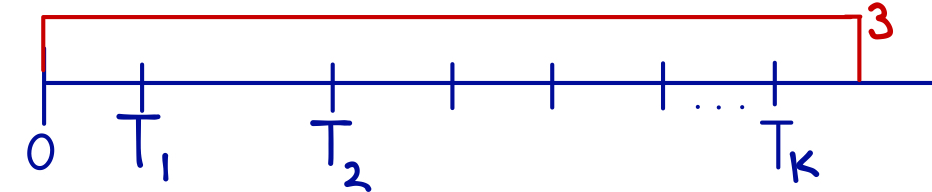
\includegraphics[height=1.4cm, width=12cm]{HW6/P2.jpeg}$$
    
    \newpage
    \item $P(N(2)=k\;|\; T_3 > 4)$
    \begin{enumerate}[label=(\roman*)]
        \item $P(N(2)=2)$
        $$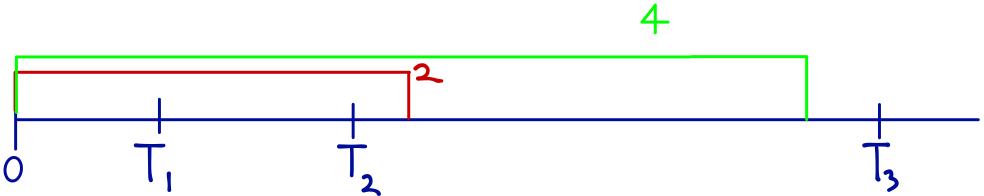
\includegraphics[height=1.4cm, width=12cm]{HW6/P1_a.jpeg}$$
        $$\frac{P(N(2)=2)\cdot P(N(4)-N(2)=0)}{P(N(4)=2)}=
        \frac{\left(\cancel{e^{-2\lambda}}\cdot \frac{(2\cancel{\lambda})^2}{\cancel{2!}}        \right)\cdot \cancel{e^{-2\lambda}}}
        {\left(\cancel{e^{-4\lambda}}\cdot \frac{(4\cancel{\lambda})^2}{\cancel{2!}}        \right)}
        =\frac{1}{4}        $$
        
        \item $P(N(2)=1)$
        $$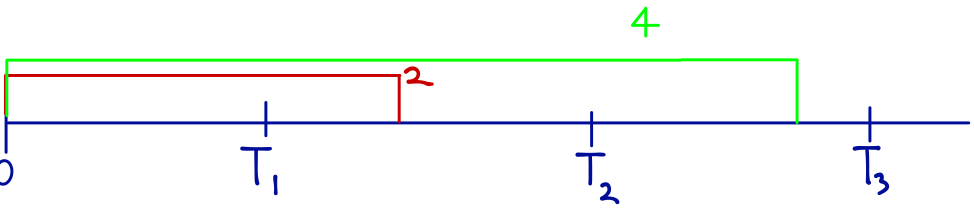
\includegraphics[height=1.4cm, width=12cm]{HW6/P1_b.jpeg}$$
        $$\frac{P(N(2)=2)\cdot P(N(4)-N(2)=1)}{P(N(4)=2)}=
        \frac{\left(\cancel{e^{-2\lambda}}\cdot \frac{(2\cancel{\lambda})^2}{\cancel{2!}}        \right)\left(\cancel{e^{-2\lambda}}\cdot \frac{(2\lambda)^1}{1!}\right)}
        {\left(\cancel{e^{-4\lambda}}\cdot \frac{(4\cancel{\lambda})^2}{\cancel{2!}}        \right)}
        =\frac{1}{2}        $$
        
        \item $P(N(2)=0)$
        $$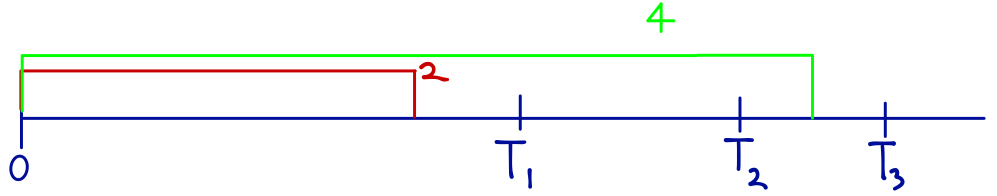
\includegraphics[height=1.4cm, width=12cm]{HW6/P1_c.jpeg}$$
        $$\frac{P(N(2)=0)\cdot P(N(4)-N(2)=2)}{P(N(4)=2)}=
        \frac{\cancel{e^{-2\lambda}}\cdot \left(\cancel{e^{-2\lambda}}\cdot \frac{(2\cancel{\lambda})^2}{\cancel{2!}}\right)}
        {\left(\cancel{e^{-4\lambda}}\cdot \frac{(4\cancel{\lambda})^2}{\cancel{2!}}        \right)}
        =\frac{1}{4}        $$
    \end{enumerate}
    
    \vspace{1\baselineskip}
    $$P(N(2)=k\;|\; T_3 > 4)=
    \begin{cases}
    1/4 & \text{if }P(N(2)=2)\\
    1/2 & \text{if }P(N(2)=1)\\
    1/4 & \text{if }P(N(2)=0)
    \end{cases}
    $$
    
    \vspace{1\baselineskip}
    \item $P(T_2\le 3\;|\; N(4)=5).$ Explain how your answer can be expressed in terms of a certain binomial probability mass function.
    $$P(T_2\le 3\;|\; N(4)=5)=
    \frac{P(N(3)=2)\cdot P(N(4)-N(3)=3)    }
    {P(N(4)=5)}    $$
    
    $$=
    \frac{\left(\cancel{e^{-3\lambda}}\cdot
    \frac{(3\lambda)^2}{2!}    \right)
    \left(
    \cancel{e^{-\lambda}}\cdot \frac{\lambda^3}{3!}
    \right) }
    {\left(\cancel{e^{-4\lambda}}\cdot
    \frac{(4\lambda)^5}{5!}    \right)}
    =
    \frac{5!}{2!\cdot 3!}\cdot
    \frac{(3\cancel{\lambda})^2\cdot \cancel{\lambda^3}}{(4\cancel{\lambda})^5    }
    =\binom{5}{3}\cdot \frac{3^2}{4^5}
    $$
    $$
    =\binom{5}{3}\cdot \left(\frac{3}{5}\right)^2\cdot \left(\frac{1}{4}\right)^3
    $$
\end{enumerate}

\newpage
{\bf 2.36 } Customers arrive at an automated teller machine at the times of a Poisson process with rate of 10 per hour. Suppose that the amount of money withdrawn on each transaction has a mean of \$30 and a standard deviation of \$20. Find the mean and standard deviation of the total withdrawals in 8 hours.


\newpage
{\bf 2.38 } Let $S_t$ be the price of stock at time t and suppose that at times of a Poisson process with rate $\lambda$ the price is multiplied by a random variable $X_i > 0$ with mean $\mu$ and variance $\sigma^2$. That is $$S_t = S_0 \prod_{i=1}^{N(t)} X_i$$ where the product is 1 if $N(t)=0$. Find $ES(t)$ and var$S(t)$. 

\vspace{1\baselineskip}
{\bf 2.44 }Ellen catches fish at times of a Poisson process with rate 2 per hour. 40\% of the fish are salmon, while 60\% of the fish are trout. What is the probability she will catch exactly 1 salmon and 2 trout if she fishes for 2.5 hours?

\vspace{1\baselineskip}
{\bf 2.48 } When a power surge occurs on an electrical line, it can damage a computer without a surge protector. There are three types of surges: “small” surges occur at rate 8 per day and damage a computer with probability 0.001; “medium” surges occur at rate 1 per day and will damage a computer with probability 0.01; “large” surges occur at rate 1 per month and damage a computer with probability 0.1. Assume that months are 30 days.
\begin{enumerate}[label=(\alph*)]
    \item What is the expected number of power surges per month?
    \item What is the expected number of computer damaging power surges per month?
    \item What is the probability a computer will not be damaged in one month?
    \item What is the probability that the first computer damaging surge is a small one?
\end{enumerate}

{\bf 2.49 }Wayne Gretsky scored a Poisson mean 6 number of points per game. 60\% of these were goals and 40\% were assists (each is worth one point). Suppose he is paid a bonus of 3K for a goal and 1K for an assist.
\begin{enumerate}[label=(\alph*)]
    \item Find the mean and standard deviation for the total revenue he earns per game.
    \item What is the probability that he has 4 goals and 2 assists in one game?
    \item Conditional on the fact that he had 6 points in a game, what is the probability he had 4 in the first half?
\end{enumerate}

{\bf 2.51 }Two copy editors read a 300-page manuscript. The first found 100 typos, the second found 120, and their lists contain 80 errors in common. Suppose that the author’s typos follow a Poisson process with some unknown rate  per page, while the two copy editors catch errors with unknown probabilities of success $p_1$ and $p_2$. Let $X_0$ be the number of typos that neither found. Let $X_1$ and $X_2$ be the number of typos found only by 1 or only by 2, and let $X_3$ be the number of typos found by both.
\end{document}